\chapter{Spherical Constraint}
In this chapter we investigate the problem in a different paradigm than what we did before.
With the aim of explicitly discriminating between norm learning and other learning steps,
we fix the value of the norm of weights at each step of the gradient descent.
A new dynamic emerges, from which, through the study of the associated differential equations,
we will derive some interesting properties of the process.

In the first section of the chapter we will give a mathematical defiition of the dynamics we will use and derive the associated differential equations.
In the next parts we will apply what we found to phase retrivial, and then generalize step by step to the case of a generic committee machine.


\section{Constrainted dynamics and differential equations}
In this section we adapt the dynamics, both for gradient descent and differential equations, to the new spherical constraint.
The derivation we present it's general and it does not assume anything on the activation function;
the results we will present will therefore be valid for any choice of activation function.
We will use the notation introduced in Chapter~\ref{chap:context}.

We start by assuming that all the weights we deal with belong to the sphere in \(d\) dimensions of radius \(\sqrt{d}\)
\[
  \vec{w}^\nu_j, \vec{w}^*_r \in S^{d-1}{\left(\sqrt{d}\right)}.
\]
The choice of radius, and hence normalization, follows from the fact that we want
the macroscopic variables to be of order 1 even in the high-dimensional limit.

In order to make valid this assumption, we have to force the norm of the student's weights to be
exactly \(\sqrt{d}\) at every step of the process. We modify the update rule as follows
\[ \w^{\nu+1}_j =\frac{\w^{\nu}_j - \gamma \nabla_{\w_j}{\loss}}{\left\|\w^{\nu}_j - \gamma \nabla_{\w_j}{\loss}\right\|}\sqrt{d}.\]
%todo: parla un po' delle varie possibilitá di gradiente e del perché alla fine abbiamo scelto questa.
We might naively think that it may suffice to take the component of the gradient tangent to the hypersphere,
and move in that direction using therefore as an update rule
\[
  \w^{\nu+1}_j = \w^{\nu}_j - \gamma \left[
    \nabla_{\w_j}{\loss} - \left(\frac{\w^{\nu}_j}{\sqrt{d}}\cdot\nabla_{\w_j}{\loss}\right)\frac{\w^{\nu}_j}{\sqrt{d}}
  \right].
\]
Unfortunately, this is not enough to maintain the spherical constraint on the weights.
The process we are analyzing is discrete, and it is the finite learning rate that causes the weights to lose the required normalization.
In order to use the gradient tangent to the surface we must take the limit \(\gamma\to0\).
This regime is known as \emph{gradient flow} and has already been used to study two-layers neural networks (in example \cite{chizat2018global}).
However, it is not what we want to study, so we will continue with the first update rule we proposed.

The update rule can be directly used for simulating the training process of a committee
machine, but it requires some work before it can be used for deriving some differential equations.
In particular, we want to find it's expansion for \(d\to+\infty\), keeping only leading orders terms.
Before proceeding to the expansion, we analize the order of single terms,
rembering the quantities we are dealing with are random variables.

We recall that the gradient is vector of random variables because of its dependence on \(\vec{x}^\nu\).
To be precise, also the displacement \(\dsp\) is a random variable, but the order of its value does not scale with \(d\),
so for our purpose it does not count. The gradient of the loss is given by
\[\nabla_{\w_j}{\loss} = -\frac{1}{p}\dsp^\nu_j \frac{\vec{x}^\nu}{\sqrt{d}}.\]
We can show that both the norm and the scalar product with a weight vector are order 1
\[\begin{split}
  \left\|\nabla_{\w_j}{\loss}\right\|^2 \sim&
    \frac{\dsp^2_j}{p^2} \frac{\sum_{i=1}^d \left(x^\nu_i\right)^2}{d}\sim
    \frac{\dsp^2_j}{p^2}\frac{\chi^2_d}{d} = \BigO{1},\\
  \w_j\cdot\nabla_{\w_l}{\loss} \sim&
    -\frac{\dsp_l}{p}\sum_{a=1}^d\frac{w_{j,a}}{\sqrt{d}}\gauss{(0,1)} \sim
    -\frac{\dsp_l}{p^2}\gauss{\left(0,\sum_{a=1}^d\frac{w^2_{j,a}}{d}\right)} \sim
    -\frac{\dsp_l}{p^2}\gauss{\left(0,1\right)}= \BigO{1}.
\end{split}\]

We are now ready to write the update rule expansion.
 Let's start by computing the the normalization factor
\[\begin{split}
  \frac{1}{\left\|\w^{\nu}_j - \gamma \nabla_{\w_j}{\loss}\right\|} =&
    \left[\left(\w^{\nu}_j - \gamma \nabla_{\w_j}{\loss}\right)\cdot\left(\w^{\nu}_j - \gamma \nabla_{\w_j}{\loss}\right)\right]^{-\frac12} \\
    =&\left[\left\|\w^{\nu}_j\right\|^2 - 2\gamma\w^{\nu}_j\cdot \nabla_{\w_j}{\loss}+\gamma^2\left\|\nabla_{\w_j}{\loss}\right\|^2\right]^{-\frac12} \\
    =&\frac{1}{\sqrt{d}}\left[1- \frac1d\left(2\gamma\w^{\nu}_j\cdot \nabla_{\w_j}{\loss}-\gamma^2\left\|\nabla_{\w_j}{\loss}\right\|^2\right)\right]^{-\frac12} \\
    =&\frac{1}{\sqrt{d}}\left[1+ \frac{1}{2d}\left(2\gamma\w^{\nu}_j\cdot \nabla_{\w_j}{\loss}-\gamma^2\left\|\nabla_{\w_j}{\loss}\right\|^2\right)+\smallo{d^{-1}}\right]
\end{split}\]
We can now plug this expansion back in the original update rule
\[
  \w^{\nu+1}_j =\left(\w^{\nu}_j - \gamma \nabla_{\w_j}{\loss}\right)\left[1+ \frac{1}{2d}\left(2\gamma\w^{\nu}_j\cdot \nabla_{\w_j}{\loss}-\gamma^2\left\|\nabla_{\w_j}{\loss}\right\|^2\right)+\smallo{d^{-1}}\right]\sqrt{d}.
\]
Let us notice that if we keep only leading terms in the learning rate we obtain 
the naive update rule we discussed above. 
This is consistent with what we have said about the gradient flow regime. 

We are ready to go over the steps that take us from the update rule on vector weights
to those on order parameters. We report by way of example the steps performed for \(\M\);
the accounts for \(\Q\) are similar, just a bit more tedious.
\[\begin{split}
  \left[\M^{\nu+1}\right]_{jr} &= \frac{\w^{\nu+1}_j\cdot\w_r^*}{d} \\
    &= \left(\left[\M^{\nu}\right]_{jr} - \frac{\gamma\w_r^*\cdot\nabla_{\w_l}{\loss}}{d}\right)\left[1+ \frac{1}{2d}\left(2\gamma\w^{\nu}_j\cdot \nabla_{\w_j}{\loss}-\gamma^2\left\|\nabla_{\w_j}{\loss}\right\|^2\right)+\smallo{d^{-1}}\right]\\
    &= \left[\M^{\nu}\right]_{jr} - \frac{\gamma\w_r^*\cdot\nabla_{\w_l}{\loss}}{d} + \frac{\left[\M^{\nu}\right]_{jr}}{2d}\left(2\gamma\w^{\nu}_j\cdot \nabla_{\w_j}{\loss}-\gamma^2\left\|\nabla_{\w_j}{\loss}\right\|^2\right)+\smallo{d^{-1}} \\
    &= \left[\M^{\nu}\right]_{jr} +\frac{1}{d}\left[
      \frac{\gamma}{p} \lf^*_r\dsp^\nu_j -
      \frac{\left[\M^{\nu}\right]_{jr}}{2}\left(2\frac{\gamma}{p}\dsp^\nu_j\lf^\nu_j + \frac{\gamma^2}{p^2} {\dsp^\nu_j}^2\right)
    \right] + \smallo{d^{-1}}.
\end{split}\]
We can now take the limit \(d\to+\infty\), claiming that the Theorem~\ref{thm:process_to_ode_goldt} is still valid.
It's not hard to belive that it is, since in the right-hand-side we have expression of the same kind
as those in the original version of the theorem; we will make the similarity explicit in a moment.
Indeed, if the hypothesis are met, than we have the same ``concentarting to mean''behaviour we have already encutered.
The differential equation that describe the evolution of \(\M\) is
\[
  \dod{\left[\M{\left(t\right)}\right]_{jr}}{t} =\E_{\vec{\lf},\vec{\lf^* \sim \gauss{(0,\vec{\Omega}{(t)})}}}{\left[\frac{\gamma}{p} \dsp_j \lf_r^* - \frac{\left[\M{\left(t\right)}\right]_{jr}}{2}\left(2\frac{\gamma}{p}\dsp^\nu_j\lf^\nu_j + \frac{\gamma^2}{p^2} {\dsp^\nu_j}^2\right)\right]};
\]
Using the definitions introduced in Equations~\eqref{eq:genericODEforM}~and~\eqref{eq:genericODEforQ} we can write the equation in a nicer form
\begin{equation} \label{eq:genericsphericalM}
  \dod{\left[\M{\left(t\right)}\right]_{jr}}{t} = \Psi_{jr}{(\vec{\Omega})} - \frac{\left[\M{\left(t\right)}\right]_{jr}}{2}\Phi_{jj}{(\vec{\Omega})}.
\end{equation}
Essentially, the spherical constraint can be imposed by using a term proportional to the unconstrainted \(\Q\) update.

Without reporting all the calculations, we can write an analougus differential equation for \(\Q\) evolution
\begin{equation} \label{eq:genericsphericalQ}
  \dod{\left[\Q{\left(t\right)}\right]_{jl}}{t} = \Phi_{jl}{(\vec{\Omega})} - \frac{\left[\Q{\left(t\right)}\right]_{jl}}{2}\left(\Phi_{jj}{(\vec{\Omega})}+\Phi_{ll}{(\vec{\Omega})}\right).
\end{equation}
Note that \(\dod{\left[\Q{\left(t\right)}\right]_{jj}}{t}=0\) if \(\left[\Q{\left(t\right)}\right]_{jj}=1\),
as it should be since the norm of spherical vectors must not change.

The two equations we derived are valid for any activation function; we can find an explicit form for the squared activation using
the expression of \(\Phi\) and \(\Psi\) we wrote in Equations~\eqref{eq:quadraticODEs}.
In Figure~\ref{fig:example-spherical} we present an example of the new dynamic
with a comparsion to the unconstrained one.
\begin{figure}
  \centering
  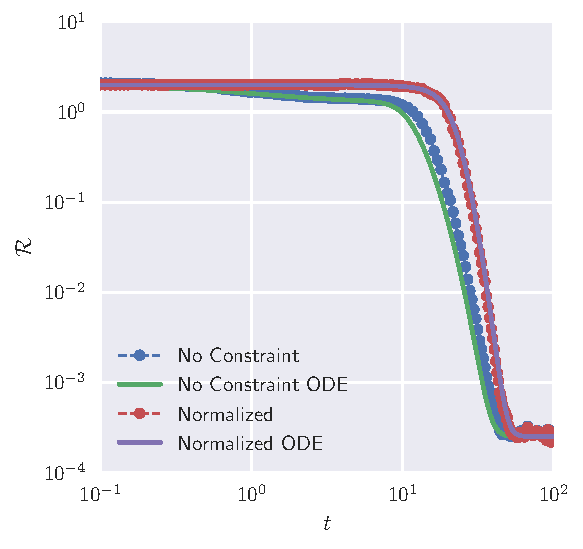
\includegraphics[width=0.7\textwidth]{figures/example-spherical.pdf}
  \caption{
    comparsion between spherical constrainted and unconstrained dynamics starting from the same intial condition.
    As we might expect in unconstrained dynamics less time is required for learning since
    there are no constraints on the gradient descent path.
    Since the simulation is not an average over several trajectories,
    it is also possible to observe the noise introduced by the stochasticity of the process;
    the constrained dynamics is less subject to noise and consequently the solution of the differential equations
    better approximates the single trajectory of the simulation.
  }
  \label{fig:example-spherical}
\end{figure}

\subsection{Initial conditions} \label{subsec:initial-condition-phaseretrivial}
We briefly discuss how to choose initial conditions.
The idea of having each component chosen randomly had removed the symmetries that prevented the differential equations from capturing all phases of the dynamics.
We would like to do the same thing in this new paradigm, but adding the spherical constraint as well.

In order to have an uniform spherical vector, it's sufficient to normalize a normal i.i.d. vector
\[
  \tilde{w}_{ji} \sim \gauss{(0,1)}\qquad\text{from which}\qquad \w_{j} = \sqrt{d}\frac{\tilde{\w}_{j}}{\left\|\tilde{\vec{w}_j}\right\|}.
\]
A completely similar initialization can be done for teacher vectors
\[
  \tilde{w}^*_{ri} \sim \gauss{(0,1)}\qquad\text{from which}\qquad \w^*_{r} = \sqrt{d}\frac{\tilde{\vec{w}}_{r}}{\left\|\tilde{\vec{w}_j}\right\|}.
\]
The set including all these vectors (both teacher and student) is nearly orthonormal in high dimension.
The diagonals of \(\Q\) and \(\P\) are all fixed to be 1. The non-diagonal terms of \(\Q\) and \(\M\) are all identicaly
distributed but only pairwise indipendent. Their distribution is the same we described for \(m(0)\) in Section~\ref{subsec:random-initial-conditions};
what interests us is that in the \(d\to\infty\) limit we can approximate it as a Gaussian with zero mean and variance \(1/d\).

\section{Phase retrivial}
Now that we have introduced the spherical constraint,
we can proceed to analyze the dynamics of learning in the simplest case: the phase retrivial.
We can use the expressions for \(\Phi\) and \(\Psi\) computed in Equations~\eqref{eq:phase_retrivial},
and plug them inside Equations~\eqref{eq:genericsphericalQ}~and~\eqref{eq:genericsphericalM} to get the 
differential equations for spherical phase retrivial dynamics.

The order parameters are reduced to a single scalar.
In fact \(\rho=1\) and \(q(t)=1\) since both \(\w\) and \(\w^*\) are constrained on the sphere.
The only variable that completely describes the process is \(m(t)\).
The differential equation for \(m(t)\) is
\begin{equation} \label{eq:spherical-phaseretrivial}
  \dod{m{(t)}}{t} = -\frac{m{(t)}}{2}\left[8\gamma(1-6\gamma)(m^2{(t)}-1)+4\gamma^2\Delta\right]\quad\text{with}\quad
  -1\le m(t)\le 1.
\end{equation}
Recalling that \(m\to-m\) symmetry applies,
we can substitute \(m\) for its absolute value without changing the description of the dynamics.

The theoreical risk is function of the only order parameter \(m\) and takes this form
\[
  \risk{(m)} = 2(1-m^2).
\]

It is clear that for the learning is all the better the more the value of \(m^2\) is close~to~1.
Without loss of generality we assume \(m>0\): for the network to learn we must impose that \(\od{m{(t)}}{t}>0\)\footnote{
  A priori one could imagine asking that the derivative always be negative, so that the value of \(m\) reaches -1.
  As we will show later, however, \(m=0\) is a repulsive fixed point of the dynamics, so it cannot be crossed.
}.
Negleting the term \(4\gamma^2\Delta\) and imposing the right-hand-side of Equation~\eqref{eq:spherical-phaseretrivial} to be positive,
we get the following condition on the learning rate
\[\gamma<\frac16 \approx \num{0.167}.\]
This condition was derived using differential equations, but it is valid as well by simulating gradient descent.
It corresponds to the empirically known fact that using too large a learning rate does not converge the algorithm to a minimum.
Figure~\ref{fig:example-spherical-not-converging} shows an example of dynamics in which the learning rate does not respect the inequality above.
\begin{figure}
  \centering
  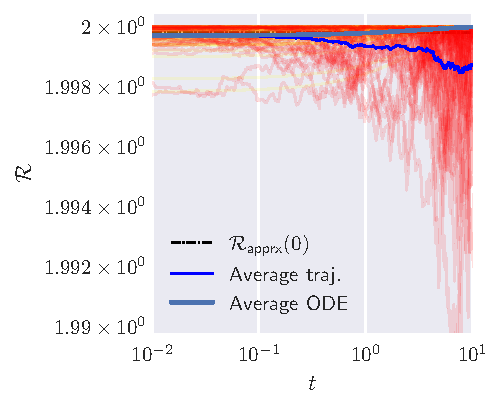
\includegraphics[width=0.6\textwidth]{figures/spherical/not-converging-phase-retrivial.pdf}
  \caption{
    example of phase retrivial with \(\gamma=0.2>\frac16, \Delta=\num{1e-3}\).\\
    As predicted, the process is not converging to a minimum, rather it stops at the maximum.
  }
  \label{fig:example-spherical-not-converging}
\end{figure}

We can now turn to analyzing how good the learning is as a function of the parameters.
Clearly, the final value of \(m{(t)}\) can only be a fixed point in Equation~\eqref{eq:spherical-phaseretrivial}.
By imposing that the derivative is zero, we find the following stationary points
\[m_{f,0} = 0 \qquad\text{and}\qquad m_{f,\pm} = \pm\sqrt{1-\frac{\gamma\Delta}{2(1-6\gamma)}}.\]
\(m_{f,0}\) is repulsive, so essentially we stay there only if we start with \(\w\) and \(\w^*\) perfectly orthogonal.
\(m_{f,\pm}\) are an attractive points and represent the same vector except for symmetry. The associated final risk is 
\[
  \lim_{t\to\infty}\risk(t) = \frac{\gamma\Delta}{1-6\gamma}.
\]
This result allowed us to formally demonstrate that the error committed on average by the student is proportional to the noise of the samples used for training.
In addition we find confirmation of another empirically known fact:
decreasing the learning rate leads to more accurate learning, even if, as we will show in a moment,
this means slowing down the process.

We can finally move to investigate the time required for learning. The average initial value of \(m{(t)}\) is given by
the same calculation we did in Section~\ref{subsec:random-initial-conditions}
\[
  \E\left[|m(0)|\right] = \sqrt{\frac{\pi}{2d}}\quad\text{and}\quad
  \E\left[m^2(0)\right] = \frac1d.
\]
In the high dimensional limit, the initial value of \(|m|\) is close to 0, so we can expand Equation~\eqref{eq:spherical-phaseretrivial} keeping only linear terms.
Solving the obtained equation give us an approximate expression for the evolution of \(m(t)\) in the first phase of the learning process.
\[\begin{split}
  \dod{|m{(t)}|}{t} =& \frac{|m{(t)}|}{2}\left[8\gamma(1-6\gamma)-4\gamma^2\Delta\right], \quad |m{(0)}| = \sqrt{\frac{\pi}{2d}} \\
  |m{(t)}| =& \sqrt{\frac{\pi}{2d}} \exp\left[\left(4\gamma(1-6\gamma)-2\gamma^2\Delta\right)t\right].
\end{split}\]
The quantity we are really interested in, however, is the theoretical risk, which depends only on \(m\).
We can therefore write its time evolution using the one just derived for \(m(t)\)
\[
  \risk_\text{apprx}{(t)} = 2\left(1-\frac1d \exp\left[2\left(4\gamma(1-6\gamma)-2\gamma^2\Delta\right)t\right]\right),
\]
where we used the same time-exponential factor as in \(m{(t)}\), but then we used \(\E\left[m^2(0)\right]\)
instead of \(\E\left[|m(0)|\right]^2\).
This choice ensures that the \(\risk(0)\) expected value is not biased,
but it may increase the variance of the trajectories thus estimated.
However, the difference factor is \(\pi/2\), which once inside a logarithm is no longer so relevant;
we will continue with our choice keeping in mind the small error it may have introduced.

Let \(T\) the relative difference respect to the initial value of the risk where the exit-time is measured.
The exit time can be obtained by solving the equation
\[
  (1-T)\risk_\text{apprx}{(0)} = \risk_\text{apprx}{\left(t^\text{(pr)}_e\right)};
\]
the final expression for the exit-time is
\[
  t^\text{(pr)}_e = \frac{\log\left[1+T(d-1)\right]}{2\left(4\gamma(1-6\gamma)-2\gamma^2\Delta\right)}.
\]
As we might have expected, the time scales logarithmically in \(d\); this in accordance with a previous result obtained 
with a completely different approach \cite{arous2021online}.
It's interesting to show how the exit-time changes as the learning rate changes.
Figure~\ref{fig:time_learnignrate_plot} shows the existence of an optimal learning rate, between 0 and the bound found above.
We emphasize that the optimality of this rate holds only in the regime in which learning has not actually started (\(m\ll1\));
in order to obtain the best final result as quickly as possible, it is necessary to implement an ad-hoc learning rate scheduling.
The result we have obtained here can be used to produce one.
\begin{figure}
  \centering
  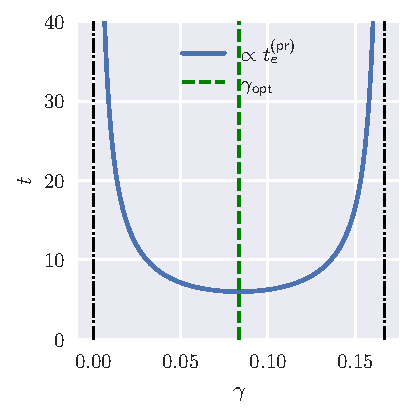
\includegraphics[width=0.55\textwidth]{figures/spherical/gamma_te-factor.pdf}
  \caption{
    plot of the exit time factor that depends on the learning rate.\\
    The optimal value for the learning rate is \(\gamma_\text{opt} = \frac{1}{12+\Delta} \approx \num{0.083}.\)
  }
  \label{fig:time_learnignrate_plot}
\end{figure}

To conclude, let us discuss the numerical experiments we performed to verify the results we have just reported.
Figure~\ref{fig:spherical-phase-retrivial-d10000} shows an example of comparsion between our results and actual simulations.
\begin{figure}
  \centering
  \begin{subfigure}{0.75\textwidth}
    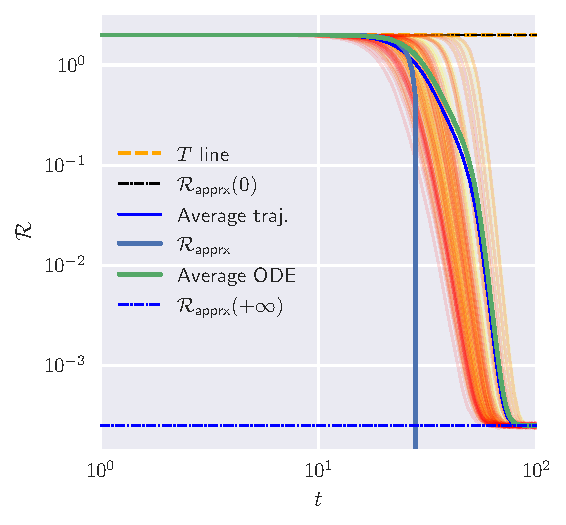
\includegraphics[width=1.\textwidth]{figures/spherical/spr-example-d10000.pdf}
    \caption{global trend}
  \end{subfigure}
  \begin{subfigure}{0.77\textwidth}
    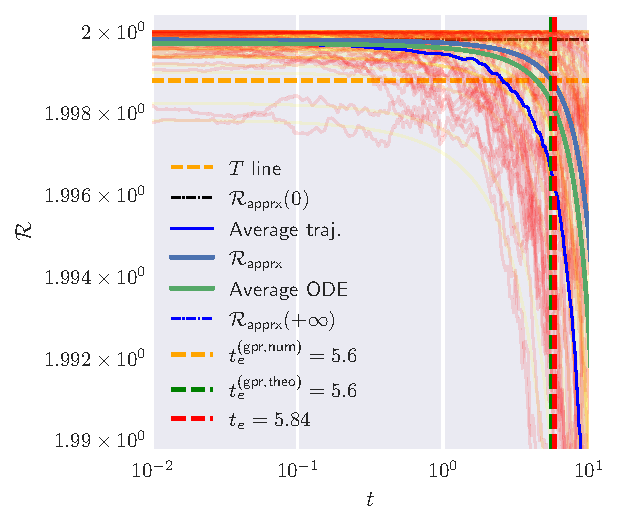
\includegraphics[width=1.\textwidth]{figures/spherical/spr-example-d10000-zoom.pdf}
    \caption{zoom}
  \end{subfigure}

  \caption{
    comparison between simulation and theory with \(\gamma=\num{0.1}, \Delta=\num{1e-3}\).\\
    The shaded red lines represent the different simulated trajectories,
    while the shaded yellow lines are the respective solutions of the differential equations.
  }
  \label{fig:spherical-phase-retrivial-d10000}
\end{figure}
We can also check whether the formula for exit-time that we derived follows the simulated trend.
Referring to Figure \ref{fig:spherical-phase-retrivial-with-d}, we see that for relatively small values of d, the formula does not work.
That is to be expected since the equations we derived hold only in the limit \(d\to\infty\).
The asymptotic trend, on the other hand, seems to have been captured correctly by the theoretical formula.
\begin{figure}
  \centering
  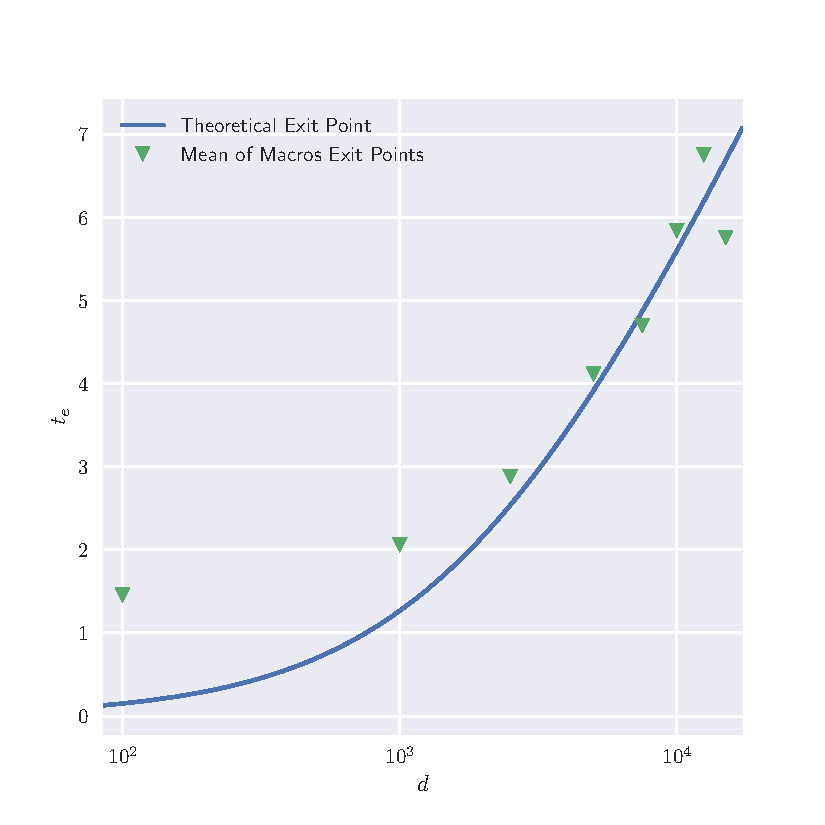
\includegraphics[width=0.9\textwidth]{figures/spherical/phase-retrivial-dplot.pdf}
  \caption{
    simulated exit time for different values of \(d\) compared to \(t^\text{(pr)}_e\).
  }
  \label{fig:spherical-phase-retrivial-with-d}
\end{figure}

\section{Generalized phase retrivial} %\label{sec:first-plateau-on-sphere}
We have just found a formula for exit time in the particular case of phase retrivial and would like to extend it to a generic committee machine.
When \(p\neq1\), in addition to the elements of \(\M\), the non-diagonal entries of \(\Q\) are also variable order parameters;
consequently, the problem becomes more complex to deal with.
We therefore decided to analyze the case \(k=1,p>1\) before moving on to the general case.
The purpose of this model is still to solve the phase retrivial,
but giving the student the opportunity to be able to mediate between different vectors \(\w_j\).

The previous section guides us in the generic case: since all the initial \(\M_j\) and \(\Q_{jl}\) are close to zero,
we can consider only the first order of the Equations~\eqref{eq:genericsphericalM}~and~\eqref{eq:genericsphericalQ}.
The full derivation is in Appendix~\ref{app:derivation-spherical-ode}; the equations are
\begin{subequations}\label{eq:genericsphericalphaseretrivial}\begin{align}
  \dod{\left[\M{\left(t\right)}\right]_{j}}{t} =&
    \left[
      \frac{4 \gamma}{p} -\frac{2 \gamma^2}{p^2} \left(2 +\frac{2}{p} + \frac{8}{p^2} + \Delta \right)
    \right] \left[\M{\left(t\right)}\right]_{j} \\
  %
  \dod{\left[\Q{\left(t\right)}\right]_{jl}}{t} =&
   -\frac{8 \gamma}{p^2} \left[1-\frac{8\gamma}{p^2}\right] \left[\Q{\left(t\right)}\right]_{jl}
\end{align}\end{subequations}
The first observation is that although the equations above represent a system of \(p(p+1)/2\) equations,
they are all independent. What follows is what is a manifestation of \emph{linear learning}: 
in the first stage of learning each hidden unit learns independently of the others.

As a second thing, we observe that again there is a maximum value of the learning rate beyond which there is no learning.
The inequality is found by imposing that \(\M=\vec{0}\) is an unstable equilibrium point of the dynamics
\[
  \frac{4 \gamma}{p} -\frac{2 \gamma^2}{p^2} \left(2 +\frac{2}{p} + \frac{8}{p^2} + \Delta \right) > 0 \quad \implies\quad
  \gamma < \frac{p}{1 +\frac{1}{p} + \frac{4}{p^2} + \frac\Delta2}.
\]
In this case we can get another inequality, by requiring that the non-diagonal \(\Q\) are deacresing in the regime we are analyzing\footnote{
  This request is not necessary, but we still ask it so that the approximate expression of theoretical risk depends on only one exponential.
  It is possible to repeat the analysis even with increasing \(q\)s, but it will not be possible to find a closed formula for exit-time.
  In any case, the inequality on \(\M\) implies that on \(\Q\) except when \(p\in[2,6]\) so the assumption is not unreasonable.
}
\[
  -\frac{8 \gamma}{p^2} \left[1-\frac{8\gamma}{p^2}\right] < 0 \quad \implies\quad
  \gamma < \frac{p^2}{8}.
\]

From Equations~\eqref{eq:genericsphericalphaseretrivial} we can find the approximated evolution of order parameters
\[\begin{split}
  \omega^{(m)}_{\gamma,p} \coloneqq \frac{4 \gamma}{p} -\frac{2 \gamma^2}{p^2} \left(2 +\frac{2}{p} + \frac{8}{p^2} + \Delta \right), \qquad
  m_j{(t)} &= m_j{(0)} \exp\left[\omega^{(m)}_{\gamma,p}t\right] \\
  %
  \omega^{(q)}_{\gamma,p} \coloneqq \frac{8 \gamma}{p^2} \left[1-\frac{8\gamma}{p^2}\right], \qquad
  q_{jl}{(t)} &= q_{jl}{(0)} \exp\left[-\omega^{(q)}_{\gamma,p}t\right]
\end{split}\]

Let's now compute the risk expression in this case. Using Equation~\eqref{eq:risk_quadratic} we get
\[
  \risk{(\Q,\M)} = 1 + \frac1p + \frac{1}{p^2}\sum_{j,l=1;j\neq l}^p q^2_{jl} - \frac2p \sum_{j=1}^p m^2_{j}
\]

As shown in Section~\ref{subsec:initial-condition-phaseretrivial}, all the \(m_j{(0)}\) and the\(q_{jl}{(0)}\) 
are random variables distributed as \(\gauss{(0,d^{-1/2})}\), in the limit of high dimension;
we can therefore compute the expecetd value and the variance of the sum of their squares
\[\begin{split}
 &\E\left[\sum_{j=1}^p m_j^2{(0)}\right] = \frac{p}{d}, \qquad
  \Var\left[\sum_{j=1}^p m_j^2{(0)}\right] = \frac{2p}{d^2}, \\
 &\E\left[\sum_{j,l=1;j\neq l}^p q_{jl}^2{(0)}\right] = \frac{p(p-1)}{d}, \qquad
  \Var\left[\sum_{j=1}^p q_{jl}^2{(0)}\right] = \frac{2p(p-1)}{d^2}. \\
\end{split}\]
We used the fact that all these variables are pairwise independent.
The distribution of these summation is becoming sharper and sharper as you go to the limit \(d\to\infty\),
so we can use the expected values for estimating \(\risk(0)\).
Combing this consideration with the approximated time evolution of the order parameters,
we can write down an approximated evolution for the risk
\[
  \risk_\text{apprx}{(t)} = 1 + \frac1p + \frac{p-1}{pd}\exp{\left[-2\omega^{(q)}_{\gamma,p} t\right]} - \frac2d \exp{\left[2\omega^{(m)}_{\gamma,p} t\right]}
\]
As we did in the previous section, we can derive an exit time by fixing a relative threshold \(T\)
and solve the equation 
\begin{equation}\label{eq:exit_time_equation}
  (1-T)\risk_\text{apprx}{(0)} = \risk_\text{apprx}{\left(t^\text{(gpr)}_e\right)}.
\end{equation}
There is no analytical solution for this equation, but we can compute the root numerically.
In order to arrive at a formula that at least approximates the solution, we will make the additional assumption 
\[
  \exp{\left[-2\omega^{(q)}_{\gamma,p} t^\text{(gpr)}_e\right]}  \approx 0,
\]
which allows us to derive this expression for the exit time
\[
  t^\text{(gpr)}_e = \frac{\log\left[\frac12+\frac{1}{2p}+\frac{T}{2}\left(1+\frac{1}{p}\right)(d-1)\right]}{\frac{8 \gamma}{p} -\frac{4 \gamma^2}{p^2} \left(2 +\frac{2}{p} + \frac{8}{p^2} + \Delta \right)}.
\]
Once again we remark the fact that the formula is scaling logarithmically in \(d\).
Figure~\ref{fig:spherical-generalized-phase-retrivial} shows two example of exit times for different \(p\).

\begin{figure}
  \centering
  \begin{subfigure}{0.75\textwidth}
    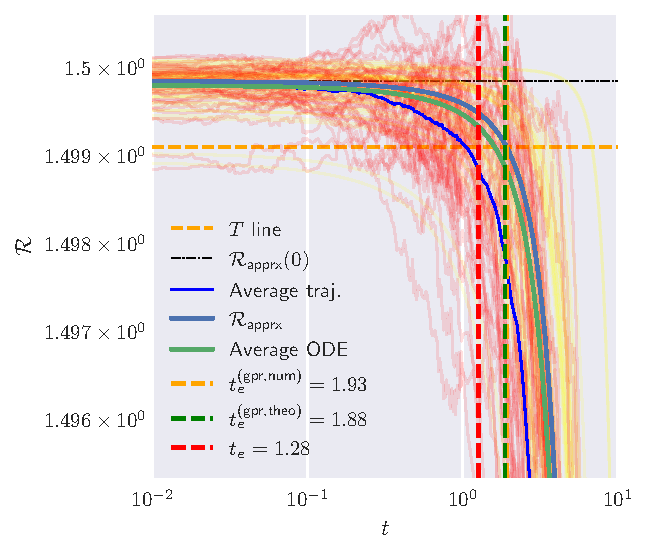
\includegraphics[width=1.\textwidth]{figures/spherical/gpr-p2.pdf}
    \caption{\(p=2\)}
  \end{subfigure}
  \begin{subfigure}{0.75\textwidth}
    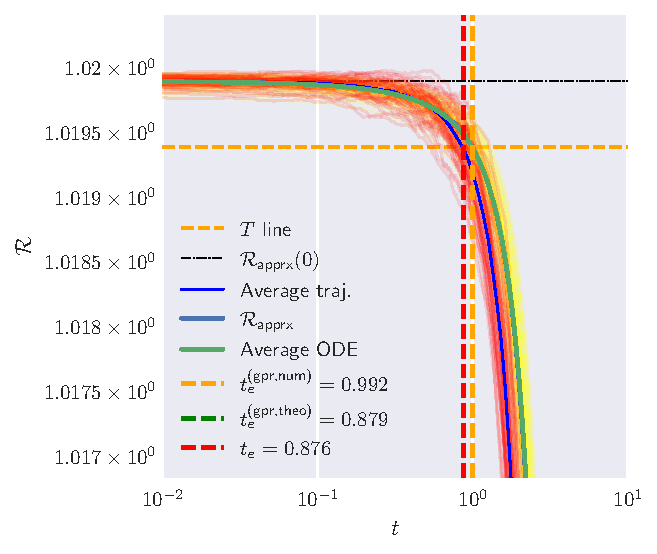
\includegraphics[width=1.\textwidth]{figures/spherical/gpr-p50.pdf}
    \caption{\(p=50\)}
  \end{subfigure}

  \caption{
    example of comparison of two exit times in the generalized phase retrivial; parameters \(\Delta=\num{0.001}, \gamma=0.2p, d=\num{10000}\).
    Both figures are zoomed in on the transition area.
    It's evident that the difference between theoretical and numerical solution of the Equation~\eqref{eq:exit_time_equation}
    is not affetcting the estimation in a significantly.
  }
  \label{fig:spherical-generalized-phase-retrivial}
\end{figure}



\subsection{Different regimes}
In this section we will try to push our result further, with the aim of deriving results on the overparametrization of neural networks.
We are aware that the formulas derived are not exact, but contain several approximations,
but we still believe they allow us to make estimates about the benefits of taking a very wide network.

The expression we derived for the exit time is valid for any fixed \(\gamma\) and \(p\).
Our final goal is to dive an empirical prove that there is a gain of performance by overparametrizing the student,
in other words taking \(p\) large. If we keep \(\gamma\) fixed, and we enlarge \(p\), the leading orderd of the exit time 
is \(t_e \propto p\). This is due to the fact that if we have \(p\) weights to learn, thre is a factor \(1/p\) in front of the gradient,
and this makes the process slow down. 

\subsubsection{Fixed $\gamma/p$}
The correct way to compare the learning between student with different \(p\) is to take the learing rate proportional to \(p\)\footnote{
  It's not a problem to enlarge the learning rate, since the update term is of order \(\frac{\gamma}{p}\BigO{1}\), so we will never have too big updates.
}.
Therefore, we define the quantity \[\alpha \coloneqq \frac{\gamma}{p},\] and we keep it costant we comparing exit times.

First of all we can derive some inequalities on the value of \(\alpha\),
which come from the inequalities we derived for the learning rate
\[\begin{split}
  \alpha <& \frac{p}{8} \quad\text{and}\\
  \alpha <& \frac{1}{1 +\frac{1}{p} + \frac{4}{p^2} + \frac\Delta2}.
\end{split}\]
As rule of dumb, if \(\alpha<\frac16\) then both this two are satisfied for every \(p\in[1,+\infty)\)\footnote{
  We remark that if \(p=1\) then the first of the two inequalities is not there since we fall back in the 
  phase retrivial case, where there are no non-diagonal \(\Q\).
}. 

Getting to the point, the expression of exit time rephrased in term of \(\alpha\) is 
\[
  t^\text{(gpr)}_e = \frac{\log\left[\frac12+\frac{1}{2p}+\frac{T}{2}\left(1+\frac{1}{p}\right)(d-1)\right]}{8\alpha} \frac{1}{1- \alpha\left(1+\frac{1}{p}+\frac{4}{p^2}+\frac{\Delta}{2}\right)}
\]
Leaving aside the logarithmic factor, whose dependence on \(p\) is practically irrelevant, 
it's clear that by incresing \(p\) we get a speedup in learning, although it is limited, and does not go to infinity as \(p\) increases.
There is a thoretical limit on the lowest time that can be achivied, even in noiseless situation, with \(p\) as large as possible.
%todo: mettici una figura di come cresce

\subsubsection{Optimal $\alpha$ at every $p$}
We have shown for phase retrivial that there is a theoretical optimal learning rate that makes the exit time minimum.
It's not hard to belive that a similar behaviour is also present in the case \(p>1\),
with a pattern of the \emph{learnig rate--exit time} curve shaped like the one in Figure~\ref{fig:time_learnignrate_plot}.
One objection to what we set forth in the previous section might be that the benefit of overparameterization is only because the increase in \(p\) brings the learning rate closer to the optimal value.
In other words, the decrease in learning time could simply be due to progressively better choice of learning rate as \(p\) changes.
In orderd to debunk this objection, we should compare the time of exists evaluated at the best possible \(\alpha\) for different \(p\).
The calculations for this part are done in this Mathematica notebook.
% todo: metti il link al notebook giusto

As we have done before, we can drop the logarithmic factor from time, keeping only this term
\[
  t{(\alpha,p)} \coloneqq \frac{1}{8\alpha\left[1- \alpha\left(1+\frac{1}{p}+\frac{4}{p^2}+\frac{\Delta}{2}\right)\right]}.
\]
We can now introduce \(\alpha_\text{op}(p)\) as the value of \(\alpha\) that minimizes the time \(t{(\alpha,p)}\) at given \(p\). 
The function \(t{(\alpha,p)}\) is \(\alpha\)-convex in the interval \((0,\alpha_\text{max})\), with \(p\) fixed;
therefore the minimum coorespond to the stationary point
\[
  0 = \eval{\dpd{t{(\alpha,p)}}{\alpha}}_{\alpha = \alpha_\text{op}(p)} \quad\text{leads to}\quad 
  \alpha_\text{op}(p) = \frac{p^2}{(2+\Delta)p^2+2 p+8}.
\]
We can now compute explicitly the best possible learning time at a given \(p\)
\[
  t_\text{opt}{(p)} \coloneqq t{\left(\alpha_\text{op}(p),p\right)} = \frac{(\Delta +2) p^2+2p+8}{4 p^2}.
\]
The most important result is that this is decrasing in \(p\), so the benefits of overparametrization are intact.
Moreover, we can also quantify the gain of overparametrizing the network as the rateo between the phase retrivial case
and the minimum time achievable
\[
  g{(\Delta)} \coloneqq \frac{t_\text{opt}{(1)}}{\lim_{p\to+\infty}t_\text{opt}{(p)}} = \frac{12+\Delta}{2+\Delta} \approx 6.
\]
Although this result is far from exact, we can still infer approximate information about the gain produced by overparameterizing the network.
In particular, we have shown that it is limited and of the order of magnitude of at most tens.
Let us emphasize again how all these results apply only to the first part of the learning;
when the network exits the initial regime, our description no longer applies and it is necessary to change the learning rate to achieve perfect learning.


\section{General Case}
We can extend our analysis to the most general committee machine, where both \(k\) and \(p\) are aribitrary.
The derivation does not include any new idea compared to the generlized phase retrivial

The diferential equations are slightly modified crespect to the prvious ones;
they are derived in Appendix~\ref{app:derivation-spherical-ode} and their final expressions are
\begin{subequations}\label{eq:cm_linearized_odes}\begin{align}
  \dod{\left[\M{\left(t\right)}\right]_{jr}}{t}
    &= \left[
      \frac{4 \gamma}{pk} -\frac{2 \gamma^2}{p^2} \left(\frac2k +\frac{2}{p} + \frac{8}{p^2} + \Delta \right)
    \right] \left[\M{\left(t\right)}\right]_{jr},\\
  \dod{\left[\Q{\left(t\right)}\right]_{jl}}{t} &= -\frac{8 \gamma}{p^2} \left[1-\frac{8\gamma}{p^2}\right] \left[\Q{\left(t\right)}\right]_{jl}.
\end{align}\end{subequations}
One again, the system of equation is fully separated, therefore the only difference between the general case and the previous one is 
the fact that \(\P\) is not a scalar, but a \(k\times k\) matrix instead. The formula for the theoretical risk is
\[
  \risk{(\Q,\M,\P)} = \frac1k + \frac1p + \frac{1}{p^2}\sum_{j,l=1;j\neq l}^p q^2_{jl} - \frac2p \sum_{j=1}^p m^2_{j} + \frac{1}{k^2}\sum_{r,t=1;r\neq t}^k \rho^2_{rt}
\]
Since \(\P\) is the teacher's eigenvector, it is a constant matrix whose entries can be estimated exactly as done with \(\Q(0)\). The initial values of the order parameters become
\[\begin{split}
  &\E\left[\sum_{j=1}^p m_{jr}^2{(0)}\right] = \frac{pk}{d}, \qquad
   \Var\left[\sum_{j=1}^p m_{jr}^2{(0)}\right] = \frac{2pk}{d^2}, \\
  &\E\left[\sum_{r,t=1;r\neq t}^k \rho_{rt}^2{(0)}\right] = \frac{k(k-1)}{d}, \qquad
   \Var\left[\sum_{r,t=1;r\neq t}^k \rho_{rt}^2{(0)}\right] = \frac{2k(k-1)}{d^2}. \\
 \end{split}\]
The approximated risk expression is 
\[
  \risk_\text{apprx}{(t)} = \frac1k + \frac1p + \frac{k-1}{kd} + \frac{p-1}{pd}\exp{\left[-2\omega^{(q)}_{\gamma,p} t\right]} - \frac2d \exp{\left[2\omega^{(m)}_{\gamma,p,k} t\right]}
\]
where \(\omega^{(q)}_{\gamma,p}\) and \(\omega^{(m)}_{\gamma,p,k}\) are properly defined from Equations~\eqref{eq:cm_linearized_odes}.

The exit time can be estimated solving Equation~\eqref{eq:exit_time_equation} with the new approximated risk.
If we want an analytical and approximate expression of the solution,
as before we can neglect the exponential in \(\Q\), yielding
\[t_e = \frac{\log \left[\frac12 + \frac{1}{2p} - \frac{T}{2k} + \frac{dT}{2k} - \frac{T}{2p} + \frac{dT}{2p} \right]}
             {\frac{8 \gamma}{pk} -\frac{4 \gamma^2}{p^2} \left(\frac2k +\frac{2}{p} + \frac{8}{p^2} + \Delta \right)}.
\]

\subsection{Overparameterization gain}
We repeat here the computation of the gain that can be achivied with overparametrization,
using the optimal learning rate at every \(p\).
The full calculations can be found on this Mathematica notebook; 
the bounds on the learning rate are not reported, but they can be found on the notebbok as well.

The optimal value of \(\alpha\) at a given \(p\) is
\[
  \alpha_\text{op}(p) = \frac{p^2}{(2+\Delta k) p^2+2 k p+8 k}
\]
and consequently
\[
  t_\text{opt}{(p)} = \frac{k \left((2+\Delta k) p^2+2 k p+8 k\right)}{4 p^2}.
\]

To conclude, this is the expression for the gain
\[
  g{(\Delta, k)} \coloneqq \frac{t_\text{opt}{(k)}}{\lim_{p\to+\infty}t_\text{opt}{(p)}} =
    \frac{\Delta k^2 + 4k + 8}{\Delta k^2 + 2k},
\]
where of course we used applied the condition \(p\ge k\).
If there is no noise, then the gain is always at least 2; 
if instead the noise it's big then there is no gain at all (even if the learning process would be so slow that the entire training it's useless).
For the last time we emphasize that these results are to be interpreted as estimates of the order of magnitude of the gain achievable by overparameterization.

In the next chapter we will try to refine our results to obtain more precise learning time estimates, but they will obviously lose analytical handling.